\section*{Nonnegative sparse coding as a modern variant of the efficient coding hypothesis}

\subsection*{Efficient coding}

The fundamental principle of \textbf{efficient coding}
is that a sensory system is
adjusted to the specific statistics of the natural environment from which
it encodes and transmits information
\cite{Barlow1961,Attneave1954,Linsker1990,LouieGlimcher2012}.

Early theories of efficient coding
\cite{Barlow1961,Attneave1954}
were developed based on the visual system.
Attneave \cite{Attneave1954} pointed out that there is a significant
degree of redundancy in natural visual images due to correlations in both
the spatial and temporal domains
(for a recent review, see \cite{SimoncelliOlshausen2001}).
For example, the luminance values of a pair of pixels
separated by a fixed distance in a natural image
are likely to be highly correlated
(Fig.~\ref{fig:ech}A).
\mikeNote{We won't be able to get CC-BY permission from SAGE. Find a different source.}
These statistical regularities constrain the images a visual system
is likely to encounter to a tiny fraction of the set of all
possible images.
It was therefore argued that the visual system should not
waste resources on processing arbitrary images,
but instead use statistical knowledge
about its environment to represent the relevant input space 
as economically as possible.


\begin{figure}[h]
	\centering
	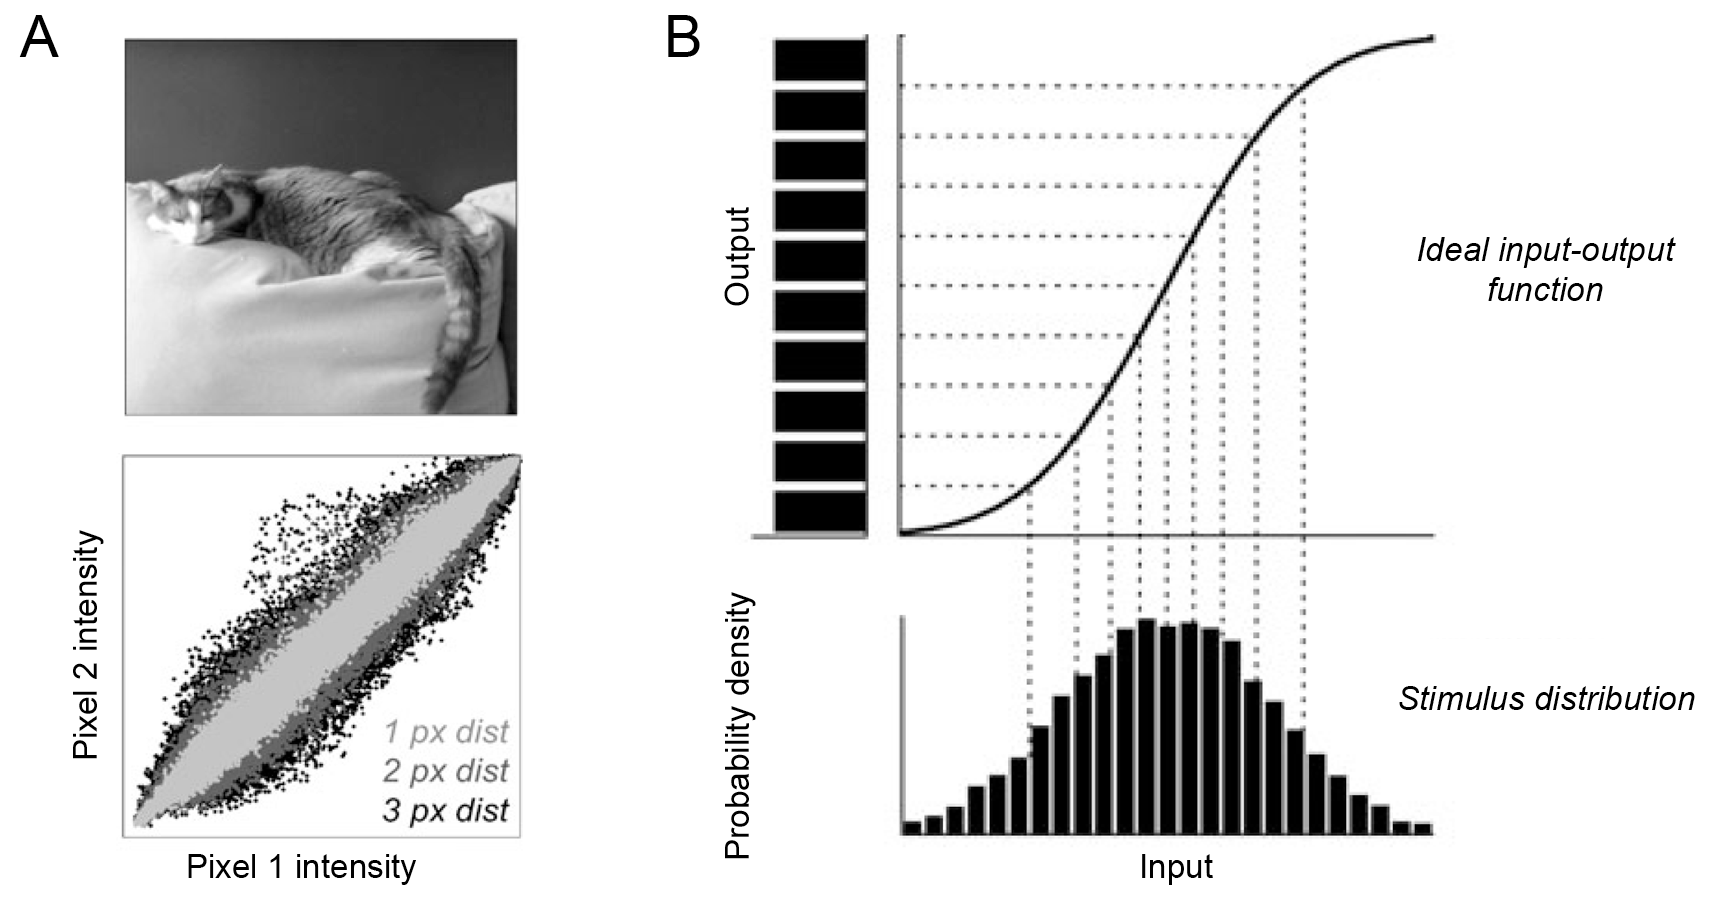
\includegraphics[width=\textwidth]{fig-rev1-ech}
    \caption{Efficient coding hypothesis.
    \textbf{\emph{A}},
         Sensory stimuli in the environment, such as an image of \revise{an anteater},
         display significant statistical structure. For example, the luminance
         value of nearby pixels in the image are significantly correlated,
         an effect that exists even for nonadjacent pixels \revise{(inspired by \cite{LouieGlimcher2012})}.
         Neural systems can improve their coding efficiency by accounting
         for and reducing such information redundancy.
     \textbf{\emph{B}},
         For a given distribution of sensory characteristics in the world (bottom),
         an efficient neural input-output function produces an output (top)
         that equally uses all possible levels of neural activity.
    }
	\label{fig:ech}
\end{figure}


Extending this idea to the neural level,
Barlow \cite{Barlow1961} proposed that
the goal of early neurons in sensory processing is to remove
the redundancy in the input stimuli.
These ideas were shaped by two
fundamental empirical observations
about early visual cortex:
1) a neuron's \ac{RF} resembled a decomposition of the visual
stimulus into a series of local, largely independent feature components
(e.g., a 2-D Gabor function is basically a local approximation of the
directional spatial derivative of an image),
and 2) any individual neuron responded only sparsely to a small subset of
stimulus features (e.g., orientation or color at a particular spatial location).
Thus a neuron's \ac{RF} could be understood as a
sparse, low-dimensional embedding of high-dimensional input stimuli
\cite{Barbieri2015}.

At the level of single neurons, efficient coding requires
that a neuron's input-output function be adjusted so that all
activity levels are used equally in response to a specific
stimulus distribution \cite{Simoncelli2003} (see Fig.~\ref{fig:ech}B).
If the input-output function sensitivity is too low,
high levels of the stimulus feature will be indistinguishable
as the response function saturates; if the sensitivity is set too high,
low levels of the stimulus feature cannot drive responses 
\cite{LouieGlimcher2012}.

At the level of neuronal populations,
neural responses should be both \emph{decorrelated}
(i.e., independent from one another)
and \emph{sparse}
(i.e., involve only a small fraction of neurons in the population)
\cite{LouieGlimcher2012}.


\subsection*{Sparse coding}

Taking these ideas a step further,
Olshausen and Field \cite{OlshausenField1996b} 
noted that natural images contain statistical
dependencies beyond linear pairwise correlations among image pixels,
and argued that these higher-order correlations should be taken into
account when developing an efficient code.
Their goal was thus to find a linear coding strategy
capable of reducing these higher-order forms of redundancy.

\emph{Linear sparse coding} is one such strategy,
where monochromatic images $I(x,y)$
are described in terms of a linear superposition of
a number of \textbf{basis functions},
$w_b(x,y)$:
\begin{equation}
I(x,y) = \sum^B_{b=1} w_b(x,y) h_b,
\label{eqn:sparse-coding}
\end{equation}
where $h_b$ are stochastic coefficients that are different for each image
\cite{OlshausenField1996,Hyvarinen2001}.
Learning a sparse code for images thus involved determining
the values of both $w_b(x,y)$ and $h_b$ for all $b$ and $(x,y)$,
given a sufficient number of observation of images,
under the constraint that $h_b$ be sparse.
In this context, $h_b$ was considered sparse if it took very small
or very large (absolute) values more often than a Gaussian random
variable would \cite{Hyvarinen2001}.
This sparsity constraint allowed for basis functions that were not
needed to describe a given image structure to be weeded out.

When Olshausen and Field applied linear sparse coding 
to natural images,
they found that the emerging basis functions 
were qualitatively similar in form
to \acp{RF} of simple cells in \ac{V1} 
\cite{OlshausenField1996,OlshausenField1997},
thus giving empirically observed \acp{RF} 
an information-theoretic explanation.
In this context, $h_b$ in Eq.~\ref{eqn:sparse-coding} above
corresponded to the (signed) activation value of a particular \ac{V1}
neuron, and $w_b(x,y)$ were the connection weights
(or \emph{synaptic weights} in an artificial neural network)
that were closely related to that neuron's \ac{RF}.
Olshausen and Field went on to show that 
the set of basis functions that best described \ac{V1} \acp{RF} 
was greater in number than the effective
dimensionality of the input (also known as an \emph{overcomplete}
basis set) \cite{OlshausenField1997}.

However, as pointed out by Hoyer \cite{Hoyer2003}, 
linear sparse coding falls short of providing a literal interpretation
for \ac{V1} simple-cell behavior for two reasons:
1) every neuron could be either positively or negatively active, and
2) the input to the neural network was typically double-signed,
whereas \ac{V1} neurons receive visual input from the \ac{LGN} 
in the form of separated, nonnegative ON and OFF channels.

In order to transform Olshausen and Field's sparse coding
from a relatively abstract model of image representation 
into a biologically plausible model of early visual cortex processing,
Hoyer \cite{Hoyer2002,Hoyer2003} thus proposed to enforce
both input signal and neuronal activation to be nonnegative.
This seemingly simple change had remarkable consequences 
on the quality of the sensory representation:
Whereas elementary image features in the standard sparse coding model
could `cancel each other out' through subtractive interactions,
enforcing nonnegativity ensured that features combined additively,
much like the intuitive notion of combining parts to form a whole.
The resulting parts-based representations resembled \acp{RF} in \ac{V1} 
much more closely than other holistic representations.
These considerations led to the formulation of nonnegative sparse coding (\ac{NSC}) in its current form.


\subsection*{Nonnegative sparse coding (NSC)}

As a special case of linear sparse coding,
\ac{NSC} shares the same goal of accurately describing observed data
as a superposition of a set of sparsely activated basis functions.
However, \ac{NSC} additionally requires 
all basis functions and activation values
(i.e., $w_b(x,y)$ and $h_b$ in Eq.~\ref{eqn:sparse-coding})
to be nonnegative.

Consider $S$ observed stimuli or data samples,
each comprised of $F$ observed feature values,
such as a collection of $S$ images $I(x,y)_s$ ($s \in [1, \ldots, S]$)
from the example above,
each consisting of $F$ different grayscale values.
If we arrange the observed feature values of the $s$-th observation into
a vector $\vec{v}_s$ (i.e., by flattening each observed image),
and if we arrange all vectors into the columns 
of a $F \times S$ data matrix \textbf{V},
then linear decompositions describe these data as:
\begin{equation}
\mathbf{V} \approx \mathbf{WH},
\label{eqn:linear-decomposition}
\end{equation}
where \textbf{W} is a $F \times B$ matrix that contains as its columns
the $B$ basis functions of the decomposition
(i.e., the $b$-th column of \textbf{W} corresponding to 
$w_b(x,y)$ $\forall x,y$ in Eq.~\ref{eqn:sparse-coding}),
and \textbf{H} is a $B \times S$ matrix containing
as its columns the activation values 
of each basis function for a particular input stimulus
(i.e., the $b$-th column of \textbf{H} corresponding to 
$h_b$ $\forall b$ in Eq.~\ref{eqn:sparse-coding}).
The difference between \textbf{V} and \textbf{WH} is termed
the \emph{reconstruction error}.

The goal of \ac{NSC} is then to find a linear decomposition of \textbf{V}
that minimizes the reconstruction error,
while guaranteeing that \textbf{H} is sparse.
This can be achieved by minimizing the following cost function
\cite{Hoyer2002}:
\begin{equation}
\min_{\mathbf{W}, \mathbf{H}} \frac{1}{2} ||\mathbf{V} -\mathbf{WH}||^2 + \lambda \sum_{ij} f(\mathbf{H}_{ij}),
\label{eqn:nsc-cost-function}
\end{equation}
subject to the constraints
$\forall ij: \mathbf{W}_{ij} \geq 0$, $\mathbf{H}_{ij} \geq 0$, and
$||\vec{w}_i|| = 1$, where $\vec{w}_i$ denotes the 
$i$-th column of \textbf{W}.
Here, the left-hand term describes the reconstruction error,
whereas the right-hand term describes the sparsity of the decomposition.
The trade-off between accurate reconstruction and sparsity
is controlled by the parameter $\lambda$ ($\lambda \geq 0$), whereas
the form of $f$ defines how sparsity is measured
(a typical choice is the L1 norm on \textbf{H}).
\revise{\Ac{NSC} explicitly discourages statistically inefficient representations,
because strongly accounting for a rare observation 
at the expense of ignoring a more common one stimulus component
would result in an increased reconstruction error.}

In the case of $\lambda = 0$, Eq.~\ref{eqn:nsc-cost-function}
reduces to the squared-error version of \ac{NMF}.
Although \ac{NMF} enforces all elements of \textbf{W} and \textbf{H}
to be nonnegative,
the resulting decomposition might not be sparse,
depending on the number of basis functions $B$.
In order to emphasize decompositions where \textbf{H} is sparse,
Eq.~\ref{eqn:nsc-cost-function} should be minimized 
with $\lambda > 0$ \cite{Hoyer2002}.

Another open parameter is the number of basis functions, $B$, 
which controls the predictive power of the model,
and must be determined empirically.
With a small number of basis functions,
\ac{NSC} is unlikely to achieve a low reconstruction error
be it in familiar contexts (training data) or in novel contexts
(held-out test data).
In this case, the error depends on the systematic bias of the model,
and the model is said to \emph{underfit} the data
(left-hand side of Fig.~\ref{fig:nsc-bias-variance-dilemma}).
With increased model complexity,
the model can learn subtle differences 
between different contexts with high accuracy,
leading to a reduced bias (training) error.
However, with increased complexity, the model is more likely to learn
patterns between training contexts that arise either from underlying noise
or from spurious correlations. As a result,
the model will respond according to
these learned patterns when a novel context is presented
(rather than according to the underlying actual relationships), 
in which case the model is said to \emph{overfit} the data
(right-hand side of Fig.~\ref{fig:nsc-bias-variance-dilemma}).
Hence, the goal of a successful model is to find the ideal compromise
in the bias-variance error trade-off \cite{Beyeler2017}
(labeled `best model' in Fig.~\ref{fig:nsc-bias-variance-dilemma}).

\begin{figure}[h]
	\centering
	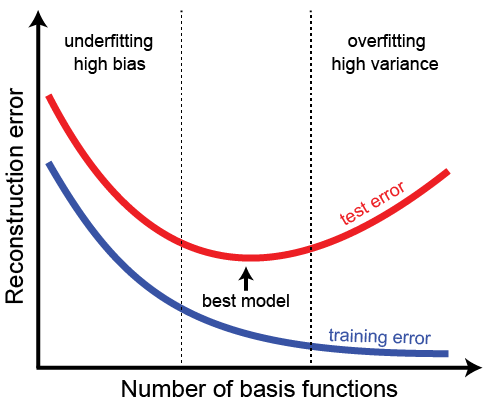
\includegraphics[width=0.6\textwidth]{fig-rev1-bias-variance}
    \caption{The bias-variance dilemma.
    With increased model complexity 
    (i.e., with an increased number of basis functions), 
    the reconstruction error on a set
    of familiar (training) data typically decreases until it reaches zero.
    In contrast, the reconstruction error on a set of unfamiliar, held-out
    (test) data typically goes through a minimum as a function of model complexity.
    A successful model chooses the number of basis functions such that the
    generalization (test) error is minimized (labeled `best model`).}
	\label{fig:nsc-bias-variance-dilemma}
\end{figure}

Analogously to \cite{OlshausenField1996,OlshausenField1997},
the basis functions obtained in \ac{NSC} can be interpreted as
the connection weights of a population of simulated neurons
in an artificial neural network.
In other words, under \ac{NSC} the number of basis functions $B$ 
corresponds to the number of output neurons, and the
response of the $b$-th model output neuron
($b \in [1, ..., B]$)
to a particular input stimulus $s$, termed $r_{bs}$,
can be computed by feeding the dot product of
that neuron's connection weights
(i.e., the $b$-th column in $\mathbf{W}$, $\vec{w}_b$)
and a data vector
(i.e., the $s$-th column in \textbf{V}, $\vec{v}_s$)
to an activation function $\Theta$:
\begin{equation}
r_{bs} = \Theta(\vec{w}_b \cdot \vec{v}_s),
\label{eqn:nsc-model-response}
\end{equation}
where $\cdot$ denotes the dot product.
For example, the linear response of a model neuron
can be calculated by setting $\Theta$ to the identity function $\Theta(x)=x$.
Note that the response of the model neuron to different stimuli 
$s \in [1, \ldots, S]$
involves different columns of \textbf{V},
but always relies on $\vec{w}_b$.

Inhibitory connections can be modeled in the same fashion,
\mikeNote{R1: maybe it’d be interesting if the authors could provide more detail into how they’d build this model with E/I neurons}
\emilyNote{What does R1 mean by "this model?" The RSC model kind of is an E/I implementation of an NMF model, as we show later, so we could just describe a random balanced network with STDP-H}
\mikeNote{I think they want to see how to build V1 cells from E/I LGN inputs. Would be good to talk about the Hoyer study or show a figure from [42].}
by interpreting inhibitory connection weights
as nonnegative synaptic conductances.
This not only preserves the parts-based quality of the encoding,
but also allows for more complicated connection types to be modeled
(e.g., \ac{V1} neurons receiving input from both excitatory ON
and inhibitory OFF cells in the \ac{LGN}) \cite{Hoyer2003}.
However, it is interesting to note that a more recent study has argued
that the nonnegativity constraint on the
connection weights might not be necessary 
to preserve the parts-based quality of the encoding \cite{Liu2017}.


Thus, we can utilize \textbf{W} 
(which must remain fixed once learned)
and Eq.~\ref{eqn:nsc-model-response}
to simulate a model neuron's response to arbitrary input stimuli
by replacing the column in \textbf{V} with new input.
This allows us to investigate the response properties 
of individual model neurons
much in the same way that experimental neuroscientists 
study biological neurons.
This is important because it means that \ac{NSC} can be used to 
model neural activity in the brain, 
and the resulting activity patterns generated by \ac{NSC}
can be compared to and evaluated against experimental findings. 

